\documentclass[../monografia.tex]{subfiles}

\graphicspath{ {images/}{../images/} } % deixei aqui pra parar de aparecer erro, tava me irritando, só comentar de volta

\begin{document}



Para o desenvolvimento do projeto, dividimos as tarefas entre 3 áreas: Hardware, Firmware e Software. 

No \textbf{hardware} estará concentrado todo o desenvolvimento da eletrônica dos dispositivos que estarão nos nós da rede. 
O \textbf{firmware} será todo o software embarcado no dispositivo, desde a comunicação com o hardware até a comunicação sem fio, entre os dispositivos da rede e do dispositivo \textit{gateway} com a plataforma. 
O \textbf{software}, por fim, trata do desenvolvimento relacionado à plataforma onde os dados serão armazenados e apresentados. 

Por fim, foi desenvolvido um case mecânico simples, impresso em 3D, para proteger os componentes. 

\section{Hardware}

A partir das especificações técnicas, foi elaborado um novo diagrama de blocos. 

\begin{figure}[h]
    \centering
    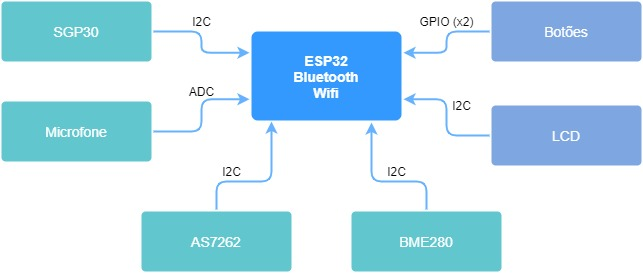
\includegraphics[width=12cm]{diagrama_hw_v1}
    \caption{Diagrama de Blocos de Hardware do Protótipo}
    \label{fig:img1}
\end{figure}

Quando possível, foram utilizados kits de desenvolvimento e módulos que nos permitisse uma validação mais rápida do hardware nessa fase inicial, permitindo avançar mais com o firmware e fazer testes em campo. 

O DevKitC do ESP32 possui integrado um USB, através do qual é possível alimentar os demais subcircuitos da placa, não existindo a necessidade de uso de bateria nessa etapa. 

\subsection{Esquemático}

Para o design do hardware, utilizamos o software de CAD de PCB \textit{Altium Designer 20} \cite{altium}. Foi utilizada a licença da empresa orientadora, sendo possível também conseguir uma licença gratuita para estudantes. Os arquivos estão disponíveis em \cite{git_hw}. 

A partir do diagrama de blocos, foi desenvolvido o esquema elétrico

\begin{figure}[h]
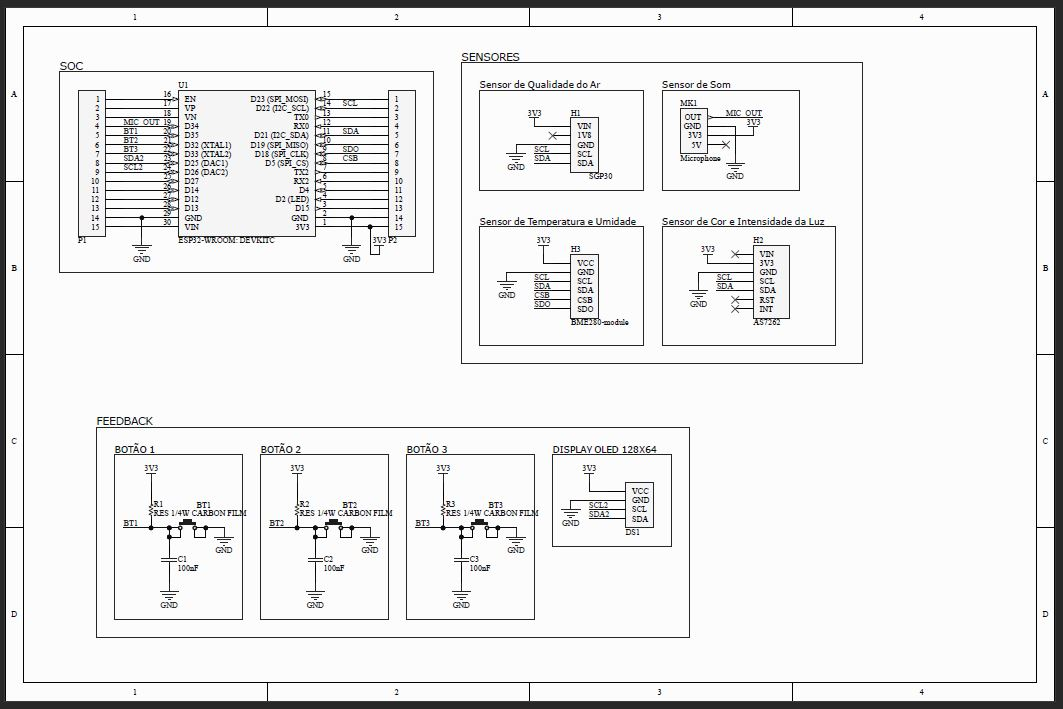
\includegraphics[width=\textwidth]{sch}
\caption{Esquemático do Protótipo}
\label{fig:img2}
\end{figure}

\subsection{PCB \textit{Printed Circuit Board}}

A partir do esquema elétrico foi feito um desenho de PCB (\textit{Printed Circuit Board}, ou Placa de Circuito Impresso), \textit{Single Layer}, e dimensões finais 60x70mm. 

\begin{figure}[h!]
\centering
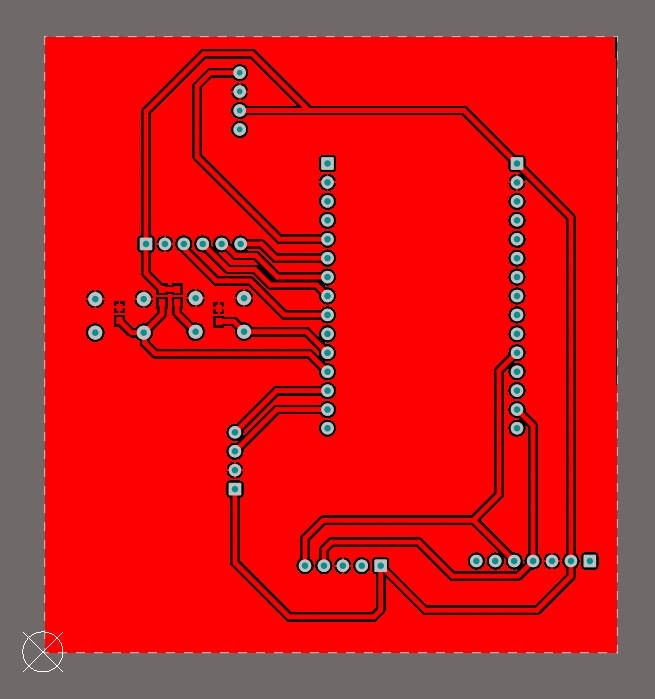
\includegraphics[width=8cm]{pcb_2}
\caption{Visão 2D da Camada Top Layer da PCB}
\label{fig:img3}
\end{figure}

%! atualizar o 3D que ta a versão 1
\begin{figure}[h!]
\centering
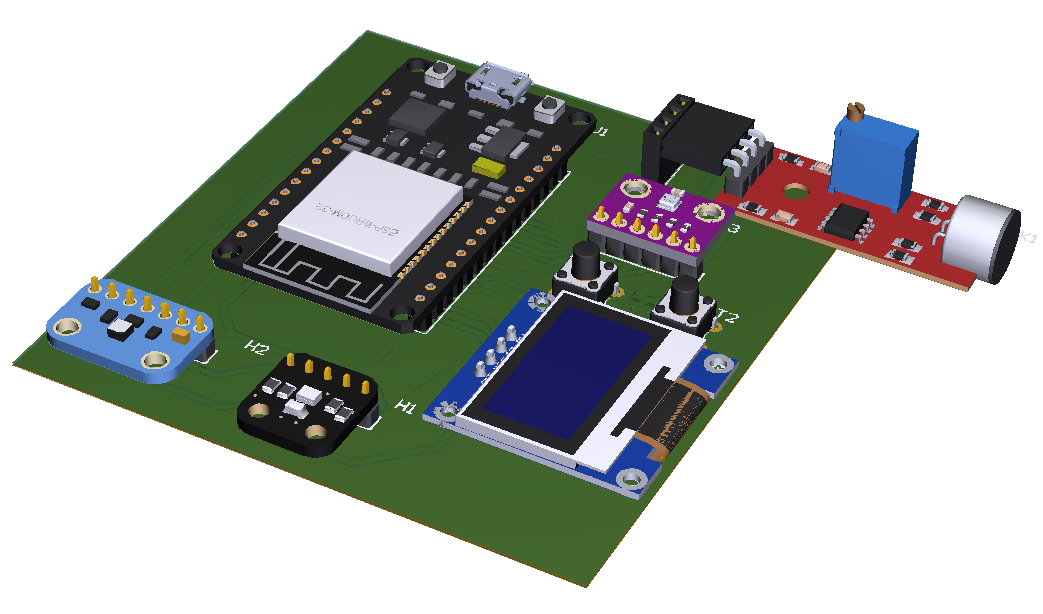
\includegraphics[width=10cm]{pcb}
\caption{Visão 3D da PCB}
\label{fig:img4}
\end{figure}

As placas foram fabricadas em fibra por uma fresadora CNC.

\begin{figure}[h!]
\centering
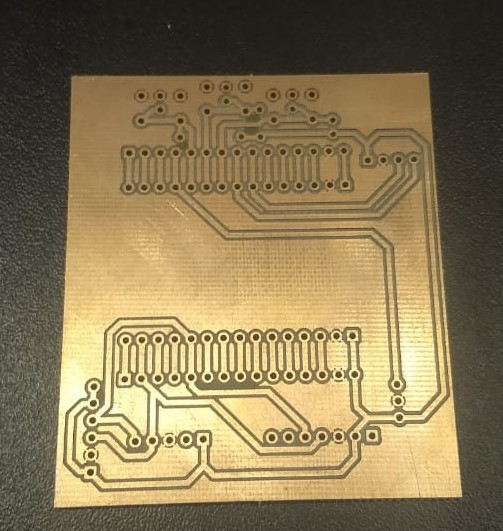
\includegraphics[width=10cm]{pcb-fresada}
\caption{PCB fresada}
\label{fig:img5}
\end{figure}

%? Montagem final da placa

\section{Firmware}

%! Pensar em como posicionar/quebrar arvore
\begin{figure}[h!]
	\centering
	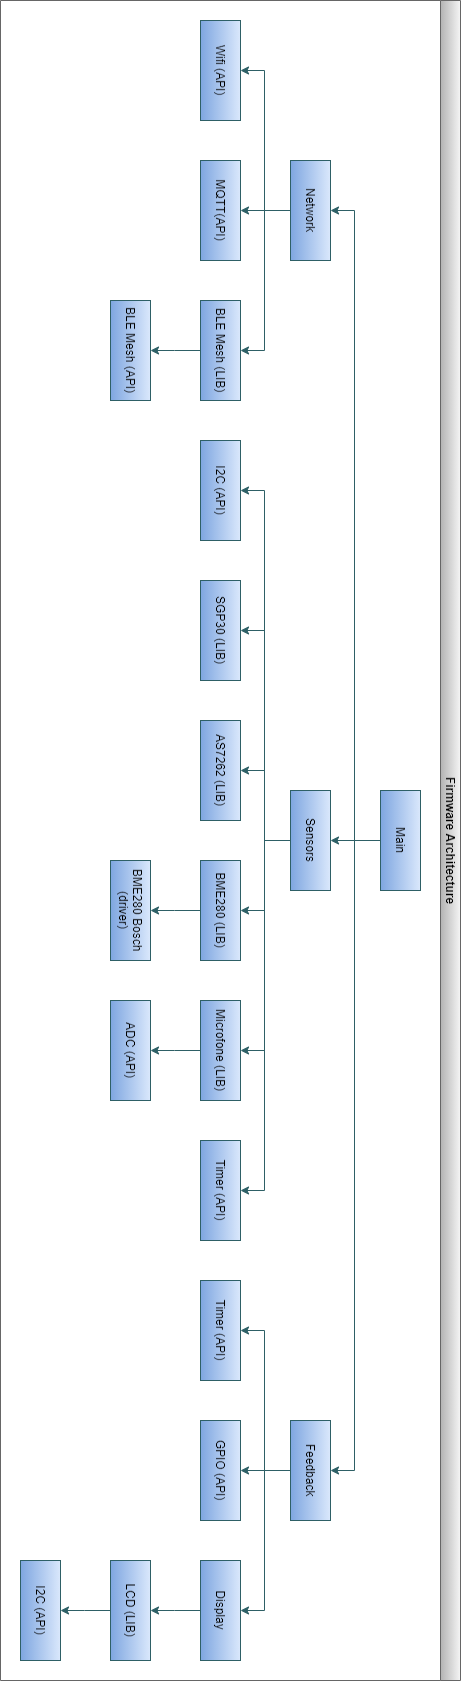
\includegraphics[height=0.9\textheight]{fw-arch}
	\caption{Arquitetura do Firmware dos dispositivos}
	\label{fig:fw-arch}
\end{figure}

\subsection{Sensores}

Para os sensores, desenvolvemos bibliotecas baseadas no ESP-IDF e validamos o funcionamento dos mesmos individualmente realizando algumas coletas de dados do ambiente. 

\subsubsection{BME280}

O BME280 é um sensor da Bosch que realiza medições de temperatura, umidade e pressão no ambiente. Possui 3 modos de operação: \cite{bme280}
\begin{itemize}
	\item \textit{sleep}: baixo consumo de energia, registradores podem ser lidos mas não realiza novas operações de medição.
	\item \textit{forced}: realiza uma medição, salva os resultados, e volta ao modo \textit{sleep}.
	
	\begin{figure}[h]
		\centering
		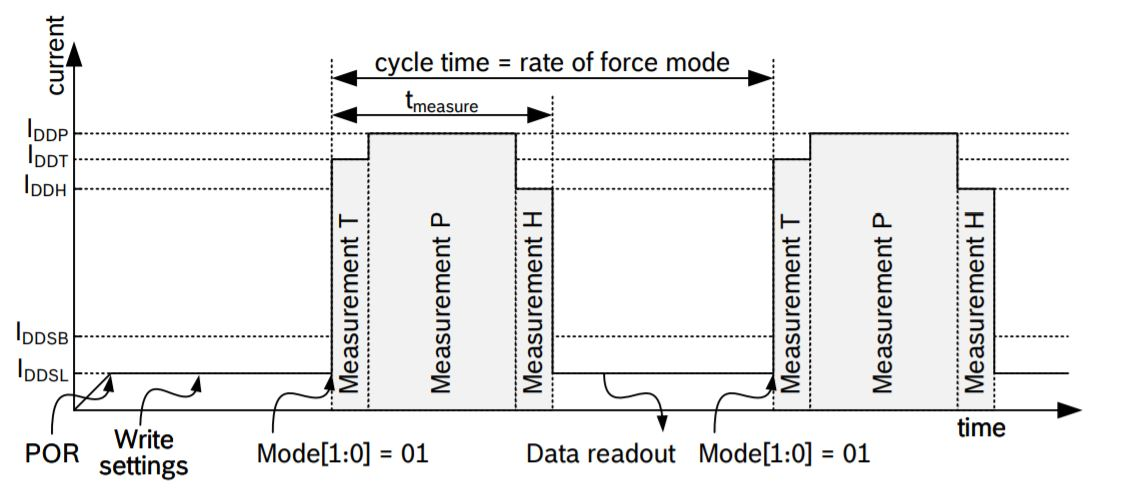
\includegraphics[width=12cm]{timing_bme280}
		\caption{Diagrama de tempos do modo \textit{forced}}
		\label{fig:time_bme280}
	\end{figure}

	\item normal: realiza medições periodicamente. O consumo durante o \textit{standby} entre medições é maior que o consumo no modo \textit{sleep}. 
\end{itemize}

O \textit{datasheet} recomenda que, para aplicações do tipo \textbf{monitoramento climático}, seja utilizado o modo \textit{forced}, com cerca de 1 medição por minuto. Assim, o sensor consumirá uma corrente de aproximadamente 0.16$\mu$A, sendo o modo de maior economia de energia. 

A Bosch Sensortech disponibiliza um driver para o BME280, com código fonte em C e disponibilizado abertamente\cite{bme280-driver}, que permite sua integração ao firmware em microcontroladores de qualquer fabricante. 
Utilizando o driver como base, desenvolvemos uma biblioteca para a utilização do BME280 no ambiente ESP-IDF, utilizando comunicação I2C, disponível

%todo: colocar estrutura da lib

%* Teste de validação 
%? manter?
% \begin{figure}[h]
% 	\centering
% 	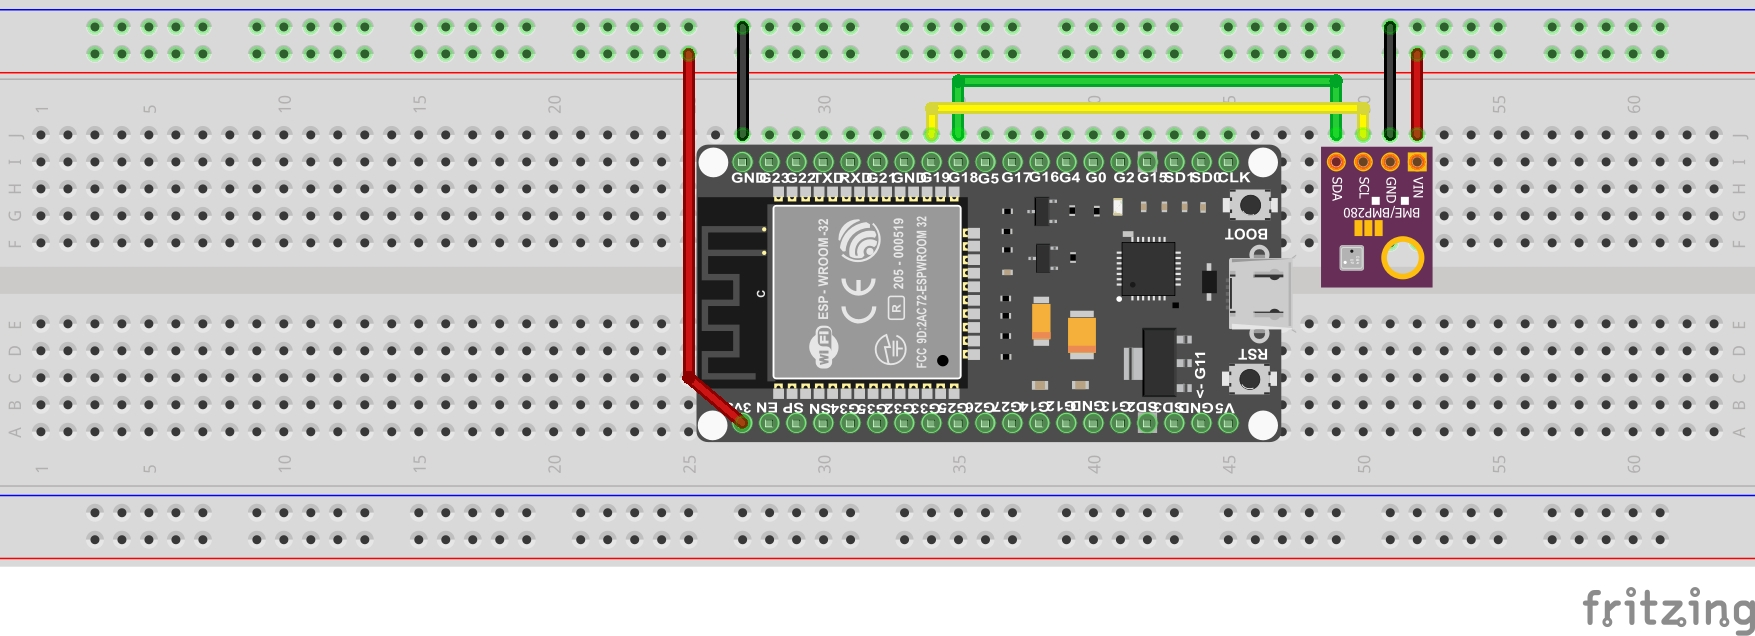
\includegraphics[width=12cm]{teste_bme280}
% 	\caption{Montagem na Protoboard do Teste com o sensor BME280}
% 	\label{fig:time_bme280}
% \end{figure}

\subsubsection{AS7262}

Para a medição de parâmetros relacionados a luminosidade, foi utilizado o sensor AS7262, da AMS, que possui filtros internos capazes de separar a luz visível de acordo com 6 comprimentos de onda: 450, 500, 550, 570, 600 e 650 nm - que correspondem às cores violeta, azul, verde, amarela, laranja e verde, respectivamente. Cada um dos filtros é lido por conversores analógico-digital de 16 bits de resolução independentes que salvam os dados em registradores internos a cada conversão realizada. Possui 4 modos de operação:

\begin{itemize}
	\item \textbf{Modo 0:} realiza medições contínuas, disponibilizando dados apenas referentes às cores violeta, azul, verde e amarela, sendo que os registradores de dados das cores vemelha e laranja ficarão com valor nulo.
	\item \textbf{Modo 1:} realiza medições contínuas, disponibilizando dados apenas referentes às cores verde, amarela, laranja e vermelha, sendo que os registradores de dados das cores violeta e azul ficarão com valor nulo.
	\item \textbf{Modo 2:} realiza medições contínuas para todos os canais.
	\item \textbf{Modo 3:} realiza medições para todos os canais, porém no modo \textit{One-Shot}.
\end{itemize}

A diferença entre os modos contínuos e o modo \textit{One-Shot} é que, no segundo, o usuário controla quando as medições deverão ser realizadas, enquanto que no modo contínuo as medições são realizadas automaticamente a partir da sua inicialização.

Outra configuração disponível para que o usuário escolha é o ganho que será aplicado nos canais de leitura, podendo ser escolhido dentre os valores 1x, 3.7x, 16x e 64x.

A interface com o sensor pode ser feita através dos protocolos I²C, utilizada nesse projeto, ou UART, através de comandos AT. Foi desenvolvida uma biblioteca na linguagem C no formato adequado para ser utilizada no ESP-IDF com a implementação das principais funções do sensor. Ao acessar o barramento I²C, só será possível visualizar 4 endereços de registradores físicos, de acordo com a tabela ~\ref{table:as7262-registers-table}.

% Please add the following required packages to your document preamble:
% \usepackage[table,xcdraw]{xcolor}
% If you use beamer only pass "xcolor=table" option, i.e. \documentclass[xcolor=table]{beamer}
\begin{table}[htp]
\begin{tabular}{|c|c|l|ll}
\cline{1-3}
\cellcolor[HTML]{C0C0C0}\textbf{Registrador} & \cellcolor[HTML]{C0C0C0}\textbf{Descrição} & \multicolumn{1}{c|}{\cellcolor[HTML]{C0C0C0}\textbf{Nota}}                                                                         &  &  \\ \cline{1-3}
\textit{Device Slave Address}                & Endereço I²C de 8 bits                     & \begin{tabular}[c]{@{}l@{}}Endereço = 1001001x (0x49), onde\\   x = 1 representa leitura\\   x = 0 representa escrita\end{tabular} &  &  \\ \cline{1-3}
STATUS                                       & Registrador de STATUS                      & \begin{tabular}[c]{@{}l@{}}Endereço 0x00\\ Sinaliza se os registradores de Leitura\\ e Escrita estão disponíveis\end{tabular}      &  &  \\ \cline{1-3}
WRITE                                        & Registrador de Escrita I²C                 & \begin{tabular}[c]{@{}l@{}}Endereço 0x01\\ \\ Valor de 8 bits a ser escrito pelo Mestre\end{tabular}                               &  &  \\ \cline{1-3}
READ                                         & Registrador de Leitura I²C                 & \begin{tabular}[c]{@{}l@{}}Endereço 0x02\\ \\ Valor de 8 bits a ser lido pelo Mestre\end{tabular}                                  &  &  \\ \cline{1-3}
\end{tabular}
\caption{Registradores físicos do sensor AS7262}
\label{table:as7262-registers-table}
\end{table}

O endereçamento dos registradores de aplicação, como os que armazenarão os dados coletados e modos de operação se dá de modo virtual. O \textit{datasheet} descreve a lógica de leitura e escrita nesses registradores virtuais:

\begin{itemize}
\item Escrita em Registrador Virtual:
	\begin{itemize}
		\item Primeiramente, ler o valor do registrador STATUS;
		\item Se o bit 1 desse registrador for igual a 0, significa que a escrita pode ser realizada;
		\item Escrever o endereço do registrador virtual no registrador WRITE (0x01) com o \textbf{MSB igual a 1} para indicar que será realizada uma escrita nele;
		\item Ler novamente o valor do registrador STATUS e verificar se o bit 1 é igual a 0;
		\item Finalmente, escrever o valor desejado para o registrador virtual no registrador WRITE.
	\end{itemize}
	
\item Leitura em Registrador Virtual:
	\begin{itemize}
		\item Primeiramente, ler o valor do registrador STATUS;
		\item Se o bit 1 desse registrador for igual a 0, significa que a escrita pode ser realizada;
		\item Escrever o endereço do registrador virtual no registrador WRITE (0x01) com o \textbf{MSB igual a 0} para indicar que será realizada uma leitura de seu valor;
		\item Ler o valor do registrador STATUS e verificar se o bit 0 é igual a 1, indicando que os dados estão prontos para serem lidos;
		\item Finalmente, ler o registrador READ (0x02), que estará com os dados requisitados.
	\end{itemize}
\end{itemize}

A lista com todos os endereços dos registradores virutais pode ser encontrada em seu \textit{datasheet} \cite{as7262}. Com essas rotinas de leitura e escrita implementadas, basta realizar a configuração desejada para a aplicação e depois ler os valores captados pelo sensor. 

\begin{figure}[h]
	\centering
	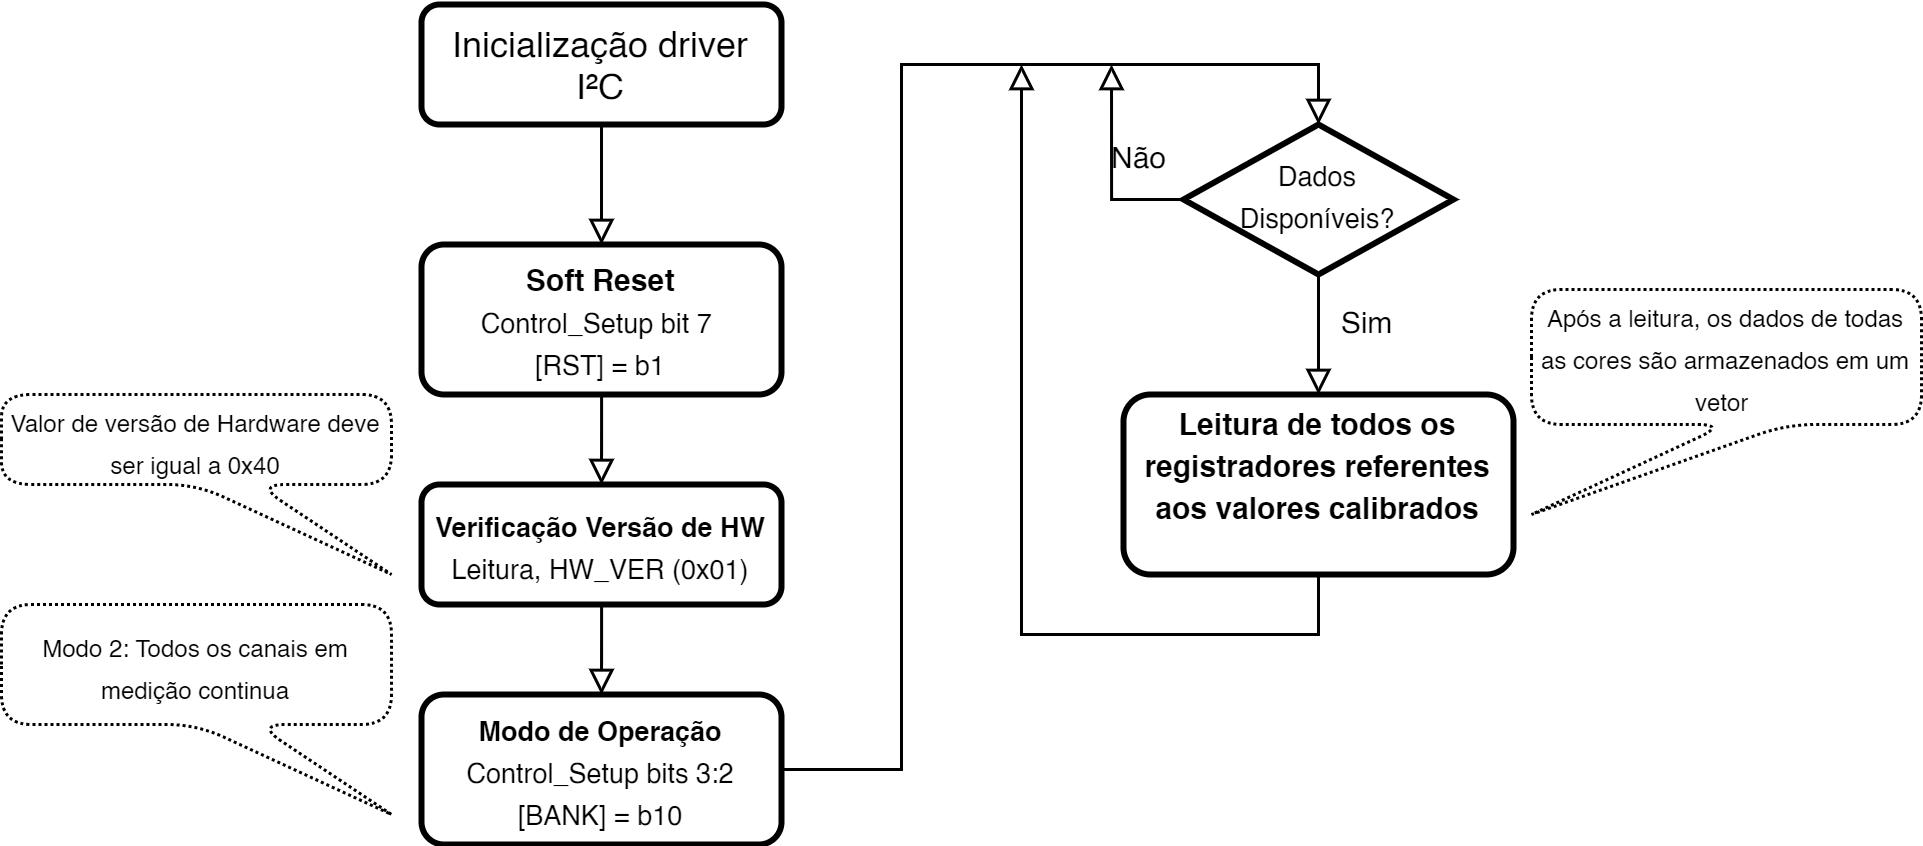
\includegraphics[scale=0.2]{as7262_firmware.png}
	\caption{Fluxograma da lógica de firmware para operação do sensor AS7262}
	\label{fig:as7262_firmware}
\end{figure}

A figura \ref{fig:as7262_firmware} mostra a lógica de aplicação implementada neste projeto. Primeiramente, é feita a operação de \textit{Soft Reset} no sensor para reinicializá-lo, depois é feita a verificação do registrador que indica a versão do Hardware, que deve ser igual a 0x40. Feita essa verificação, escreve-se o valor 0b10 para inicializar a captação de valores no \textbf{Modo 2}: modo contínuo, referentes a todos os canais de medição. O valor de cada canal será armazenado em 4 registradores, totalizando 32 bits de valores em notação de ponto flutuante para cada canal. A etapa final da aplicação é realizar a leitura desses 24 registradores (4 por canal, 6 canais no total) e salvá-los em um vetor de 6 posições, para que possam ser manipulados posteriormente.

A bilbioteca desenvolvida para a interação com o sensor pode ser acessada em \cite{as7262-lib}.

%!!!!!!!!!!!!!!!! Precisa escrever sobre interpretação dos dados


\subsubsection{SGP30}

O sensor utilizado para medições dos parâmetros referentes à qualidade do ar foi o SGP30, da Sensirion. A partir de medições de concentracão de hidrogênio e etanol no ar, um algoritmo interno ao sensor consegue estimar o total de componente orgânico volátil (TVOC), em partes por bilhão (ppb), e o equivalete de $CO_{2}$, em partes por milhão (ppm), presentes no ambiente. 

A interface com esse sensor também é feita através do protocolo I²C, porém através de comandos pré-definidos, presentes nas páginas 9 e 10 do \textit{datasheet} \cite{sgp30}. Cada comando é identificado por um valor de 16 bits e é responsável por realizar uma ação no sistema, como inicializar, realizar medições e ler valores fixados, como número de série. 

Todos os dados enviados e recebidos pelo sensor contém ao final, além dos valores padrão, 8 bits de valores para verificação cíclica de redundância (do inglês \textit{Cyclic Redundancy Check}, CRC), com a finalidade de validar os dados sendo transmitidos, utilizando o método de \textit{checksum}, calculado com o seguinte polinômio: $CRC = 0h31 (x_{8} + x_{5} + x_{4} + 1)$ - em que $x_{i}$ corresponde ao i-ésimo bit do valor utilizado para o cálculo. Os comandos de 16 bits tabelados já incluem os campos do CRC em sua composição, não sendo necessário calculá-los.

Portanto, para realizar interações com o sensor, o usuário deve realizar os seguintes passos:

\begin{itemize}
	\item Inicializar a comunicação I²C com o sensor, que possui endereço 0x58, indicando ação de escrita;
	\item Enviar o valor referente ao comando que deseja ser executado (normalmente valores de 16 bits);
	\item Alguns comandos realizam respostas, como o comando \textit{Measure\_air\_quality} (0x2008). Se o comando realizado for desse tipo, basta reiniciar a comunicação I²C, agora indicando uma ação de leitura para o endereço 0x58, que os dados requisitados estarão disponívels;
	\item Os dados de reposta virão com 8 bits de CRC ao final. O usuário pode fazer a checagem desse valor, calculando o CRC de acordo com os valores da resposta para validar os dados lidos.
\end{itemize}


Para realizar a interação com esse sensor e obter os dados necessários para esse projeto, também desenvolvemos uma biblioteca nos mesmos moldes do ESP-IDF, em linguagem C, disponível em \cite{sgp30-lib}. A rotina principal de coleta de dados é exemplificada na figura \ref{fig:sgp30_firmware}. O \textit{datasheet} indica que, para a correta inicialização do algoritmo que calcula as estimativas de $eCO_{2}$ e TVOC, é necessário que o usuário realize 14 medições espaçadas de 1 segundo, nas quais o sensor retornará valores fixos de $TVOC = 0$ e $eCO_{2} = 400 ppm$. Após esse período, o sensor começará a responder com valores válidos referentes ao ambiente em questão.

\begin{figure}[h]
	\centering
	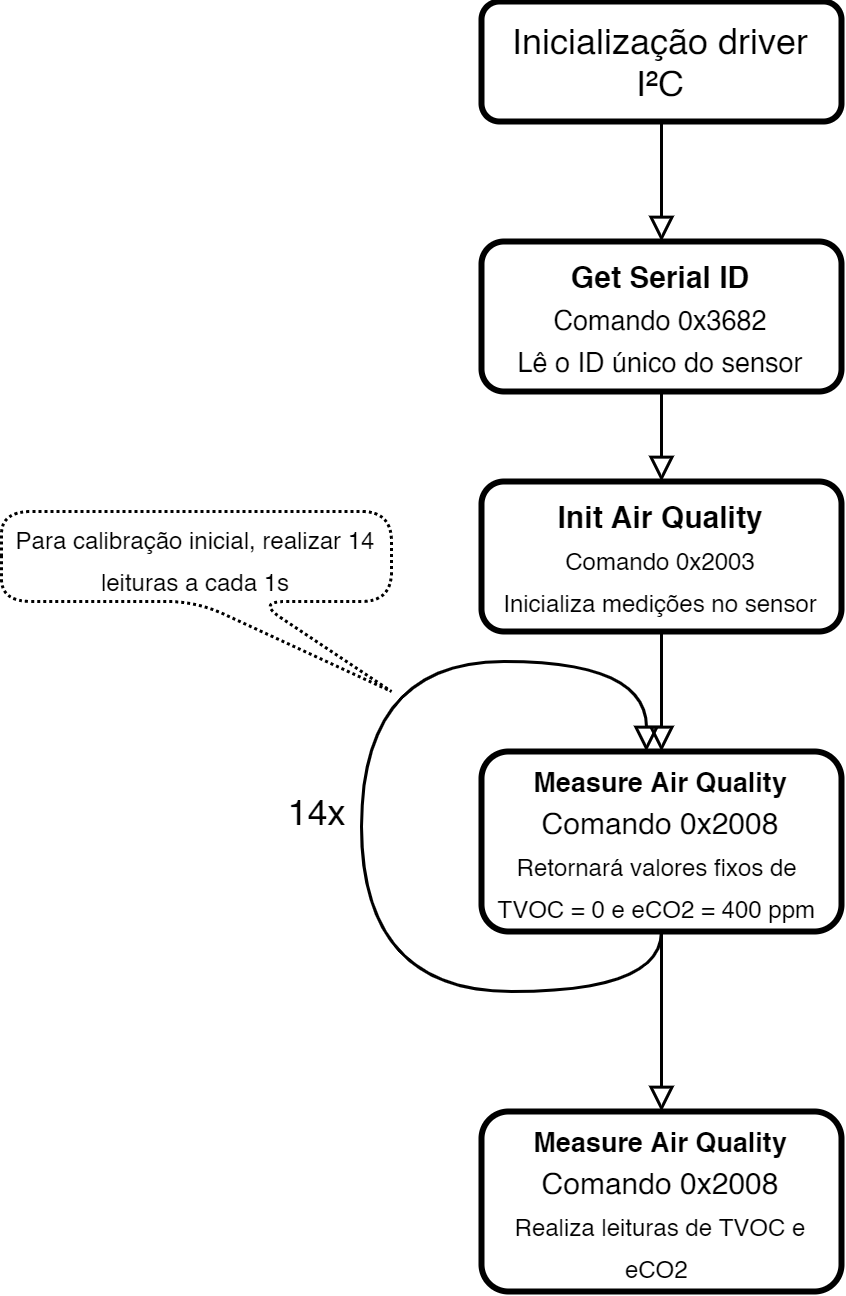
\includegraphics[scale=0.2]{sgp30_firmware.png}
	\caption{Lógica de execução de firmware para coleta de dados do sensor SGP30}
	\label{fig:sgp30_firmware}
\end{figure}

Os valores retornados pelo comando \textit{Measure Air Quality} são salvos em duas variáveis de 16 bits, a serem manipulados posteriormente.

\subsubsection{Microfone}
\subsection{Feedback}
\subsubsection{LCD OLED}
\subsubsection{Máquina de Estados}

Para a coleta do feedback, foi implementada a seguinte máquina de estados, seguindo um \textit{table-driven approach}.

%Máquina de Estados

%Estrutura do Código

\subsection{Bluetooth}
\subsubsection{Validação da Rede Mesh}

Visando validar a parte de comunicação sem fio utilizando BLE Mesh do ESP32 para o uso no projeto, uma rede simples com apenas 3 dispositivos foi desenvolvida. Dentre os dispositivos, 2 deles eram constituídos pelo microcontrolador escolhido conectados a de 3 LEDs cada um, e o terceiro um \textit{smartphone}. 

\begin{figure}[h]
	\centering
		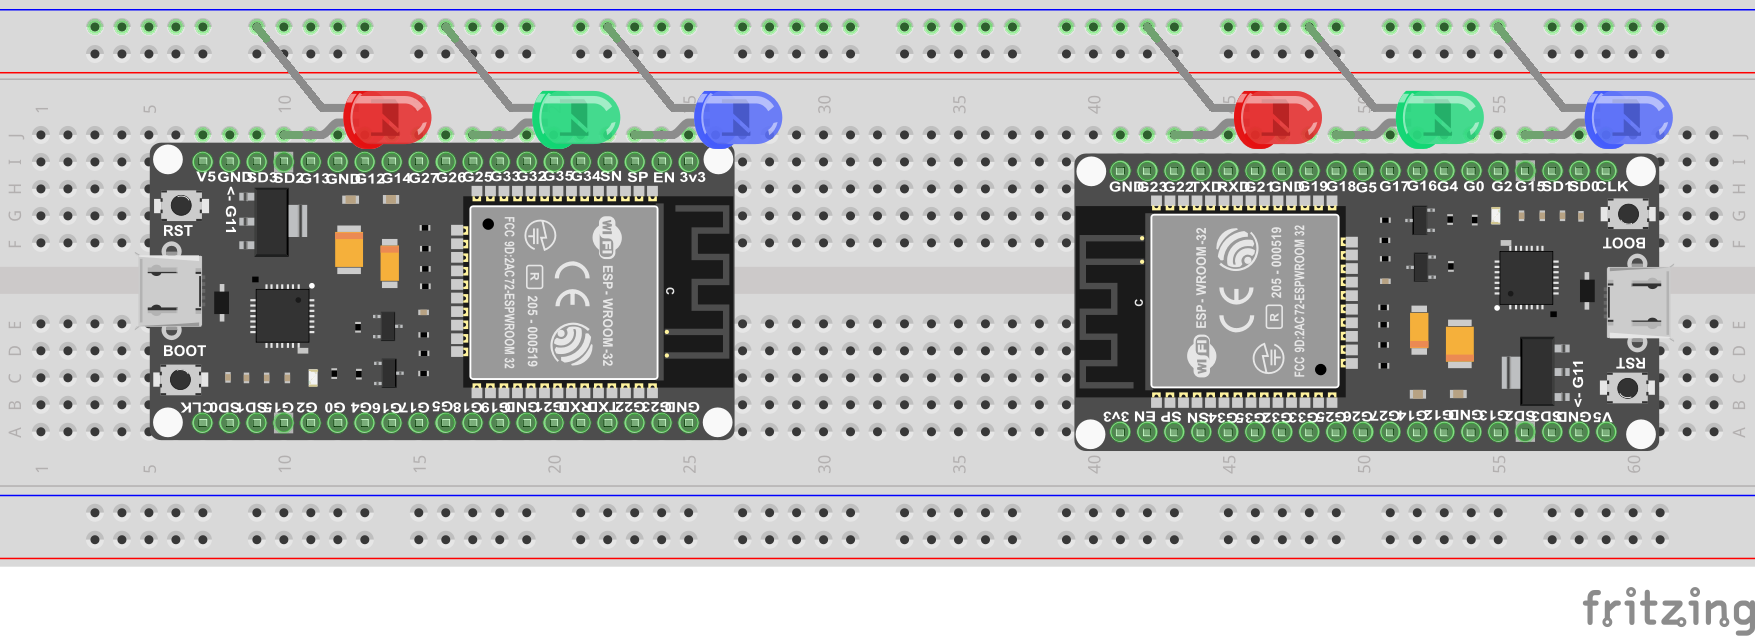
\includegraphics[width=.8\textwidth]{mesh_test}
		\label{fig:test}
		\caption{Montagem na Protoboard para o teste de Validação da Rede Mesh}
\end{figure}

Arquitetura da rede de testes criada:

\begin{itemize}
	\item Nó com microcontrolador ESP32: 3 elementos, cada um com o \textit{OnOff Server Model} \cite{ble-mesh-models} implementado, visando controlar o ligamento e desligamento de um LED.
	\item \textit{Smartphone}: utilizando o aplicativo nRF Mesh \cite{nrf-app}, usado para provisionar os outros nós e controlar a rede \textit{mesh}.
\end{itemize}

O teste completo aqui descrito pode ser visto em \cite{teste-ble-mesh}.

A partir do aplicativo citado, os outros dois dispositivos foram provisionados, criando a rede \textit{mesh}. Depois, foram criados 3 grupos diferentes:

\begin{itemize}
	\item \textit{Red Lights}: grupo em que os \textit{models} que controlam os LEDs vermelhos nos nós foram inscritos;
	\item \textit{Green Lights}: grupo em que apenas um dos \textit{models} que controlam LEDs verdes foi incrito;
	\item \textit{Red and Blue}: grupo em que tanto os \textit{models} de LEDs vermelhas quanto os de LEDs azuis foram inscritos.
\end{itemize}

O funcionamento da rede pode ser validado quando mensagens de \textit{On} e \textit{Off} eram enviadas em cada grupo e apenas os LEDs que deveriam receber a mensagem do respectivo grupo era acionado ou desligado.

Foi possível visualizar o a criação e o funcionamento de uma rede BLE Mesh na plataforma escolhida, bastando apenas modificar a lógica e parâmetros necessários para que as mensagens contenham os dados coletados pelos sensores do projeto e sejam enviadas para os dispositivos desejados.

\subsection{Wifi}
\subsubsection{MQTT}
\section{Software}
\section{Mecânica}

Foi projetado um case mecânico para proteger a eletrônica dos dispositivos, a ser impresso em 3D. 

O case é composto por duas peças, uma base, onde fica fixada a placa, e uma tampa onde ficam fixados o display OLED e os botões. As laterais abertas permitem que sejam feitos ajustes dos módulos com sensores sem afetar o funcionamento destes. 

\begin{figure}[h]
	\centering
	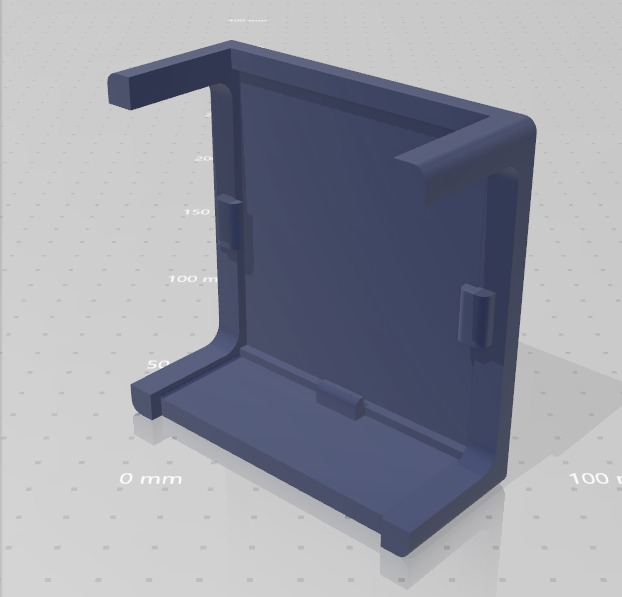
\includegraphics[width=0.6\textwidth]{mec-base.jpeg}
	\caption{Base do Case Mecânico}
	\label{fig:mec1}
\end{figure}

\begin{figure}[h]
	\centering
	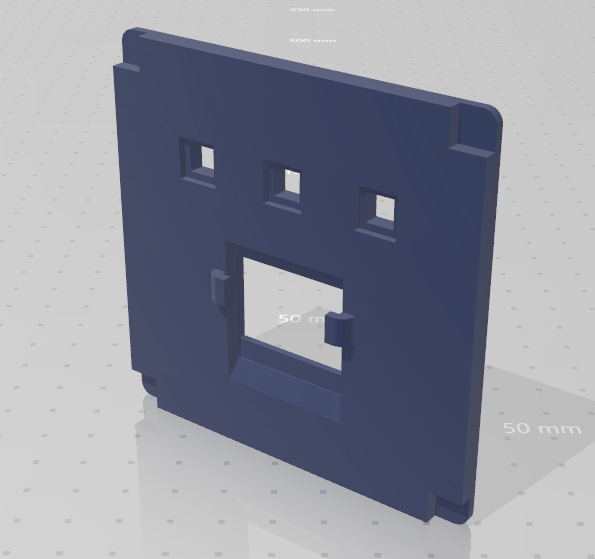
\includegraphics[width=0.6\textwidth]{mec-tampa.jpeg}
	\caption{Tampa do Case Mecânico}
	\label{fig:mec2}
\end{figure}

%* Montagem Final com Case

\end{document}